\chapter{Results}
\label{chap:results}
% - Results
%    - the cli-tutor tool (result of engineering work)
%       - future work
%    - user study
%       - analysis

%%TODO: Should i just rewrite the RQs here as a reminder to the reader. Is that bad form?

%%%%%
% RQs 
%
% Are there identifiable patterns of difficulty when it                                  
% comes to adopting CLIs? Can the `indimidation factor' be pinned down? \label{rq:1}     

% How should an interactive learning tool be designed to mitigate                        
% the difficulty and indimidation factor of learning CLIs? \label{rq:2}                  

% How can a `forgiving' shell be implemented on top of an existing                       
% shell to enable the transition from learning to real-world usage? \label{rq:3}         

% Is the interactive tool more effective than text based learning methods? \label{rq:4}  

% Are novice CLI users more likely to continue                                           
% using CLI interfaces after using such a tool? \label{rq:5}                             

In this chapter, we will discuss the outcomes of this thesis work. We will look
into our findings in light of the research questions we defined in
\autoref{chap:intro} in \autoref{subsec:rqs}. Furthermore, we will divide our
results into two distinct sections, focusing on the results of the engineering
effort in building \textit{CLI-Tutor} and secondly, the findings from the user
study discussed in the preceding chapter.


\section{Engineering Results}

From an engineering perspective, we managed to achieve almost all the
technical goals we set out for \textit{CLI-Tutor}. Design goals relating to
ease of distribution and access were fulfilled as \textit{CLI-Tutor} is a single binary that
is easy to distribute and containerise. \textit{CLI-Tutor} also works natively
on  \textit{GNU/Linux} and  \textit{Macintosh} operating systems and thanks to
the associated web application and docker images for the tool, it is possible
to use \textit{CLI-Tutor} on almost any mainstream operating system. The web
application and ease of containerisation also helped achieve another goal of
creating a safe and forgiving sandboxed environment for users to experiment
within.

This ease of experimentation and application of learnt skills is an
important factor when it comes to developing confidence with CLIs as they are a
foreign interaction paradigm to most novices. Ease of experimentation and
ability to apply learnt skills is not purely achievable through technical
design alone. The curriculum of \textit{CLI-Tutor} also reflects an emphasis on
giving the user space to try things out without worry or the tutorial software
actually getting in the way. One participant in the user study particularly
admired this aspect of \textit{CLI-Tutor}: 

\begin{quotes}
	"I think the cli-tutor really provides the right amount of guidance, while
	leaving enough freedom to experiment and test things. Thus it was trivial to
	examine small questions one asks themselves like:  what would happen if one
	calls "rmdir" on a directory that contains another empty directory.  All in all
	a great experience, and a drastic improvement compared to non-interactive  2
	hour lectures."
\end{quotes}

Based, on feedback received by participants in the user study we can conclude
that the curriculum was well received and appropriately designed as many
respondents found this to be a particularly strong aspect of
\textit{CLI-Tutor}.

\begin{quotes}
	"Very good tutorial, great work! It starts at the beginning and fills the gaps
	that are necessary to make working with the command line more quicker and more
	useful."
\end{quotes}

\begin{quotes}
	"It was overall very well structured. I feelt like the tutorial was a very
	smooth process, taking you from one topic to the most closely related next
	topic."
\end{quotes}

\begin{quotes}
	"Great work, short but precise! I would love to do more of your tutorials :)"
\end{quotes}

The level of difficulty was also appropriate as many participants found the
course content appropriate for newcomers. This is encouraging as tutorial tools
are generally targeted at beginners and \textit{CLI-Tutor} is no exception.

\begin{quotes}
	"Was a pleasent and well thought out lesson. Would recommend this for newcomers
	to the CLI, as it does have a friendly and fun tone to the entire teaching
	environment."
\end{quotes}

There were also multiple participants who particularly enjoyed the interactive
aspect \textit{CLI-Tutor}. This was of particular interest to use given our a
major intention of our research was to assess the effectiveness of interactive
learning tools for the command line.

\begin{quotes}
	"The cli-tutor made it really easy for me to learn how to use the command line
	in an uncomplicated way. The interactive part was the best part about the tool.
	It required me to directly put my understanding into practice, making the
	learning process very convenient."
\end{quotes}

\begin{quotes}
	its very nice. i think there is a lot of learning when u actually have to type in stuff than just
	passivly reading. i know from myself than i need to write stuff down to learn, so beeing forced
	to type in stuff to get in another level helps me.
\end{quotes}

Even when interactive styled learning was not the preference of the participant,
as is the case with the participant below. They still were able to find some
merits in the interactive approach.

\begin{quotes}
	"i personally prefer to acquire knowledge first and then put it into practice on my own. but i
	think interactive learning is a very effective method for many people to learn new things.
	especially when it comes to something that triggers fear of contact (for example the cli, or git).
	the cli-tutor is a really cool tool, visually and in terms of content! the most important things are
	repeated more than once, and repetitions are very important for the learning effect."
\end{quotes}

\subsection{Relevant Research Questions}

\ref{rq:2} and \ref{rq:3} are technically orientated research questions. Based
on what we learnt in the feedback provided by participants in the user study we
will now provide some insights into potential answers to these research questions.


\paragraph{\ref{rq:2}.} \textit{How should an interactive learning tool be designed to mitigate
	the difficulty and intimidation factor of learning CLIs?}

Based on the feedback received during the user study, it can be said that in
order to build effective interactive learning tools the structure and content
of lessons are of high importance. The correct sequencing, building up and
repetition of examples are key to creating an effective curriculum. Allowing
room for exploration and experimentation are other important aspects of an
effective interactive learning tool. To some participants the ability to
directly try out the lesson content made for a stronger learning experience.


\paragraph{\ref{rq:3}.} \textit{How can a `forgiving' shell be implemented on top of an existing
	shell to enable the transition from learning to real-world usage?}

The approach taken by \textit{CLI-Tutor} based on its reception seems to be
promising. Creating an intermediary between the user and the shell allowed for
tailoring the environment specifically to beginners while still being able to
be faithful to the shell interaction experience. Wrapping the shell also enabled
safety measures like not allowing the user into the sensitive root level
directories, which contributes to the safety aspect and reduces the overall
intimidation factor. The sandboxing approach takes this point and pushes it
even further as then the users have no fears of any potential negative
consequences to their systems.



\section{User Study Results}

\subsection{Evaluation section}

The following subsection, addresses research question \ref{rq:4}: \textit{Is
	the interactive tool more effective than text based learning
	methods?}

As mentioned in \autoref{chap:userstudy}, the evaluation section of our user
study is what we used to evaluate the effectiveness of the lessons our study
participants took. Since the content of all the lessons was exactly the same
across both interaction mediums this offers a reasonable way to focus
our comparison on only the interaction mediums.

A question-by-question breakdown of the percentage of correct responses per
question for both user groups is shown in \autoref{tab:evaluation}. When
averaged across all questions in the evaluation section, the interactive group
performed 9.34\% better than their non-interactive counterparts. When looking
deeper at the differences in performance there was an observable trend.
Individuals who took the interactive version of the tutor seemed to score
significantly higher on questions that related to topics that contained lots of
interactive examples in \textit{CLI-Tutor}. This is especially true for
questions relating to flags and the file system which consisted of many
interactive examples.

For a visual representation of the differences between both participant groups
in the evaluation section (see: \autoref{fig:eval}).

\subsection{Discussion}

Despite the positive results, the higher level of performance cannot be
conclusively attributed to the interaction medium alone. There are factors such
as existing experience, outliers and a small study size that must be considered
when analysing these results. However, given that the performance of the
interactive group was comparatively higher on more interactively practised
topics in the tutor, there appears to be a correlation between practise and
success when it comes to the command line.

\begin{table}[htbp]
\centering
\begin{tabular}{|c|c|c|}
\hline
\textbf{Question}                                                                                                                                                           & \begin{tabular}[c]{@{}c@{}}CLI-Tutor \\ Correct \%\end{tabular} & \begin{tabular}[c]{@{}c@{}}Non Interactive \\ Correct \%\end{tabular} \\ \hline
\textbf{\begin{tabular}[c]{@{}c@{}}Which one of the following best describes\\  the role of flags when issuing a command?\end{tabular}}                                     & 7.47                                                            & 13.28                                                                 \\ \hline
\textbf{\begin{tabular}[c]{@{}c@{}}Which one of the following best describes\\  the role of flags when issuing a command?\end{tabular}}                                     & 82.6                                                            & 29.0                                                                  \\ \hline
\textbf{\begin{tabular}[c]{@{}c@{}}Which one of the following flow diagrams\\  best describes textual interaction with \\ the operating system using a shell?\end{tabular}} & 98                                                              & 2                                                                     \\ \hline
\textbf{\begin{tabular}[c]{@{}c@{}}Which of the following is an incorrect\\ usage of flags?\end{tabular}}                                                                   & 4                                                               & 95                                                                    \\ \hline
\textbf{What is the role of the prompt?}                                                                                                                                    & 4                                                               & 97                                                                    \\ \hline
\textbf{\begin{tabular}[c]{@{}c@{}}What is the command to see where you \\ are on your file system and what\\  does the abbreviation stand for?\end{tabular}}               & 4                                                               & 99                                                                    \\ \hline
\textbf{\begin{tabular}[c]{@{}c@{}}Which of the following structures \\ describes the file system best?\end{tabular}}                                                       & 3                                                               & 3                                                                     \\ \hline
\textbf{\begin{tabular}[c]{@{}c@{}}What command do you use to list\\  the contents of your current directory?\end{tabular}}                                                 & 3                                                               & 3                                                                     \\ \hline
\textbf{\begin{tabular}[c]{@{}c@{}}Can you explain in what situations the \\ rmdir command will not delete a directory?\end{tabular}}                                       & 2                                                               & 3                                                                     \\ \hline
\textbf{\begin{tabular}[c]{@{}c@{}}What shell keyboard shortcut \\ cancels a command or input?\end{tabular}}                                                                & 2                                                               & 2                                                                     \\ \hline
\textbf{\begin{tabular}[c]{@{}c@{}}What is the name of the command that\\  brings up documentation about a command?\\  What does this command stand for?\end{tabular}}      & 2                                                               & 2                                                                     \\ \hline
\end{tabular}
\caption{Summary of questions answered correctly by method during the evaluation phase.}
\label{tab:questionsummary}
\end{table}


\begin{figure}[htbp]
	\centering
	\scalebox{0.87}{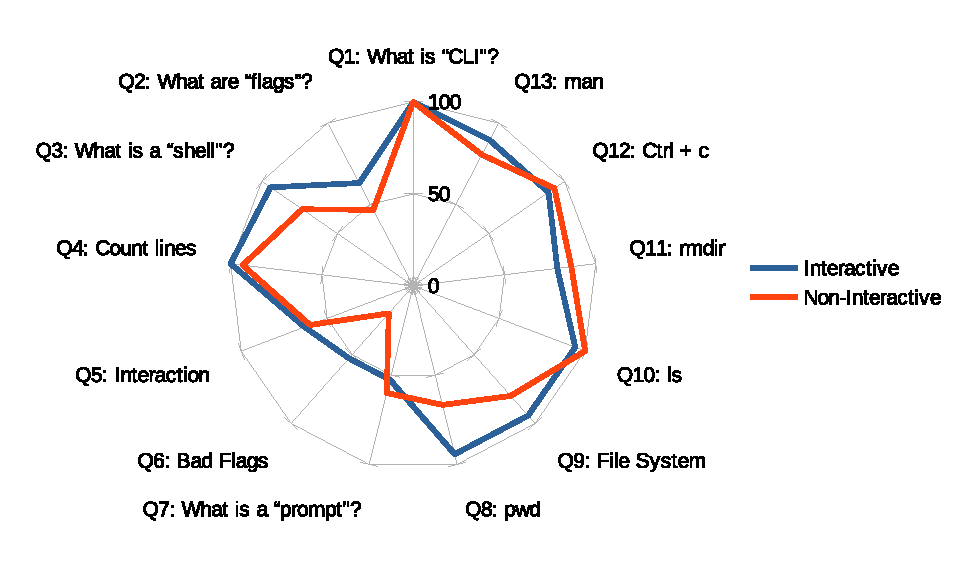
\includegraphics{plots/evalspider/spider.eps}}
	\caption{Chart depicting the evaluation section results of the interactive and non-interactive participant groups.}
	\label{fig:eval}
\end{figure}

\FloatBarrier %TODO: SEE IF THIS IS NECESSARY

\subsection{Intimidation Factors}

In the user study, participants were asked about intimidation factors regarding
command line usage to better understand the difficulties faced by
beginners in order to further improve \textit{CLI-Tutor} and any other future
research in the area of making command line interfaces more approachable.


\paragraph{\ref{rq:1}.} \textit{Are there identifiable patterns of difficulty when it comes to
	adopting CLIs? Can the `intimidation factor' be pinned down?}

Based on the results from the feedback sections of the user study, we can say
based on the data that individuals who used the interactive \textit{CLI-Tutor},
on average, left less intimidated than their non-interactive tutor
counterparts. As shown in \autoref{fig:confidence}, a mere 5.26\% of
respondents assigned to the interactive group reported feeling more intimidated
after their experience with \textit{CLI-Tutor}. On the non-interactive side
this figure was considerably higher with 26.67\% of respondents reporting
being more intimidated by the command line after the user study.

In terms of identifiable patterns of difficulty and intimidation factors,
participants were asked to identify their personal intimidation factors. Responses
included fears about lack of safety mechanisms or unintentional errors.

\begin{quotes}
	"irreversible actions"
\end{quotes}

\begin{quotes}
	"something fatal happens that I didn't want to to (something like rm without wanting it/typos/...)"
\end{quotes}

One of the most often cited intimidation factors was related to the mental overhead of remembering all the commands.
\begin{quotes}
	"If you don't use it that often, the overwhelming number of commands makes it difficult to use."
\end{quotes}

\begin{quotes}
	remembering all the things to write in order to give the command correctly
\end{quotes}

\begin{quotes}
	difficult to memorise the command and flags, especially when I'm not using them frequently
\end{quotes}

One participant even feared that the memorisation requirements might even
nullify any potential productivity gains of using the command line.

\begin{quotes}
	not knowing the commands by heart and needing to look it up (taking more time in the
	process)
\end{quotes}

Additionally, there was also mention of the unfamiliarity with command line
interfaces as an additional intimidation factor.

\begin{quotes}
	unfamiliar setting, no overview
\end{quotes}


\begin{figure}[htbp]
	\centering
	\scalebox{0.67}{%% Creator: Matplotlib, PGF backend
%%
%% To include the figure in your LaTeX document, write
%%   \input{<filename>.pgf}
%%
%% Make sure the required packages are loaded in your preamble
%%   \usepackage{pgf}
%%
%% Also ensure that all the required font packages are loaded; for instance,
%% the lmodern package is sometimes necessary when using math font.
%%   \usepackage{lmodern}
%%
%% Figures using additional raster images can only be included by \input if
%% they are in the same directory as the main LaTeX file. For loading figures
%% from other directories you can use the `import` package
%%   \usepackage{import}
%%
%% and then include the figures with
%%   \import{<path to file>}{<filename>.pgf}
%%
%% Matplotlib used the following preamble
%%   \usepackage{fontspec}
%%   \setmainfont{DejaVuSerif.ttf}[Path=\detokenize{/home/spam/miniconda3/envs/mpl/lib/python3.10/site-packages/matplotlib/mpl-data/fonts/ttf/}]
%%   \setsansfont{DejaVuSans.ttf}[Path=\detokenize{/home/spam/miniconda3/envs/mpl/lib/python3.10/site-packages/matplotlib/mpl-data/fonts/ttf/}]
%%   \setmonofont{DejaVuSansMono.ttf}[Path=\detokenize{/home/spam/miniconda3/envs/mpl/lib/python3.10/site-packages/matplotlib/mpl-data/fonts/ttf/}]
%%
\begingroup%
\makeatletter%
\begin{pgfpicture}%
\pgfpathrectangle{\pgfpointorigin}{\pgfqpoint{8.799314in}{3.116660in}}%
\pgfusepath{use as bounding box, clip}%
\begin{pgfscope}%
\pgfsetbuttcap%
\pgfsetmiterjoin%
\pgfsetlinewidth{0.000000pt}%
\definecolor{currentstroke}{rgb}{0.000000,0.000000,0.000000}%
\pgfsetstrokecolor{currentstroke}%
\pgfsetstrokeopacity{0.000000}%
\pgfsetdash{}{0pt}%
\pgfpathmoveto{\pgfqpoint{0.000000in}{0.000000in}}%
\pgfpathlineto{\pgfqpoint{8.799314in}{0.000000in}}%
\pgfpathlineto{\pgfqpoint{8.799314in}{3.116660in}}%
\pgfpathlineto{\pgfqpoint{0.000000in}{3.116660in}}%
\pgfpathlineto{\pgfqpoint{0.000000in}{0.000000in}}%
\pgfpathclose%
\pgfusepath{}%
\end{pgfscope}%
\begin{pgfscope}%
\pgfsetbuttcap%
\pgfsetmiterjoin%
\definecolor{currentfill}{rgb}{0.501961,0.694118,0.827451}%
\pgfsetfillcolor{currentfill}%
\pgfsetlinewidth{1.003750pt}%
\definecolor{currentstroke}{rgb}{1.000000,1.000000,1.000000}%
\pgfsetstrokecolor{currentstroke}%
\pgfsetdash{}{0pt}%
\pgfpathmoveto{\pgfqpoint{3.894914in}{1.314902in}}%
\pgfpathcurveto{\pgfqpoint{3.894914in}{1.442534in}}{\pgfqpoint{3.869773in}{1.568924in}}{\pgfqpoint{3.820931in}{1.686841in}}%
\pgfpathcurveto{\pgfqpoint{3.772088in}{1.804757in}}{\pgfqpoint{3.700494in}{1.911906in}}{\pgfqpoint{3.610245in}{2.002155in}}%
\pgfpathcurveto{\pgfqpoint{3.519995in}{2.092404in}}{\pgfqpoint{3.412847in}{2.163998in}}{\pgfqpoint{3.294931in}{2.212841in}}%
\pgfpathcurveto{\pgfqpoint{3.177014in}{2.261683in}}{\pgfqpoint{3.050624in}{2.286824in}}{\pgfqpoint{2.922992in}{2.286824in}}%
\pgfpathcurveto{\pgfqpoint{2.795361in}{2.286824in}}{\pgfqpoint{2.668970in}{2.261683in}}{\pgfqpoint{2.551054in}{2.212841in}}%
\pgfpathcurveto{\pgfqpoint{2.433138in}{2.163998in}}{\pgfqpoint{2.325989in}{2.092404in}}{\pgfqpoint{2.235740in}{2.002155in}}%
\pgfpathcurveto{\pgfqpoint{2.145491in}{1.911906in}}{\pgfqpoint{2.073896in}{1.804757in}}{\pgfqpoint{2.025054in}{1.686841in}}%
\pgfpathcurveto{\pgfqpoint{1.976211in}{1.568924in}}{\pgfqpoint{1.951070in}{1.442534in}}{\pgfqpoint{1.951070in}{1.314902in}}%
\pgfpathcurveto{\pgfqpoint{1.951070in}{1.187271in}}{\pgfqpoint{1.976211in}{1.060880in}}{\pgfqpoint{2.025054in}{0.942964in}}%
\pgfpathcurveto{\pgfqpoint{2.073896in}{0.825048in}}{\pgfqpoint{2.145491in}{0.717899in}}{\pgfqpoint{2.235740in}{0.627650in}}%
\pgfpathcurveto{\pgfqpoint{2.325989in}{0.537401in}}{\pgfqpoint{2.433138in}{0.465806in}}{\pgfqpoint{2.551054in}{0.416964in}}%
\pgfpathcurveto{\pgfqpoint{2.668970in}{0.368121in}}{\pgfqpoint{2.795361in}{0.342980in}}{\pgfqpoint{2.922992in}{0.342980in}}%
\pgfpathcurveto{\pgfqpoint{3.050624in}{0.342980in}}{\pgfqpoint{3.177014in}{0.368121in}}{\pgfqpoint{3.294931in}{0.416964in}}%
\pgfpathcurveto{\pgfqpoint{3.412847in}{0.465806in}}{\pgfqpoint{3.519995in}{0.537401in}}{\pgfqpoint{3.610245in}{0.627650in}}%
\pgfpathcurveto{\pgfqpoint{3.700494in}{0.717899in}}{\pgfqpoint{3.772088in}{0.825048in}}{\pgfqpoint{3.820931in}{0.942964in}}%
\pgfpathcurveto{\pgfqpoint{3.869773in}{1.060880in}}{\pgfqpoint{3.894914in}{1.187271in}}{\pgfqpoint{3.894914in}{1.314902in}}%
\pgfpathmoveto{\pgfqpoint{2.922992in}{1.314902in}}%
\pgfpathmoveto{\pgfqpoint{3.894914in}{1.314902in}}%
\pgfpathlineto{\pgfqpoint{3.894914in}{1.314902in}}%
\pgfpathclose%
\pgfusepath{stroke,fill}%
\end{pgfscope}%
\begin{pgfscope}%
\pgfsetbuttcap%
\pgfsetmiterjoin%
\definecolor{currentfill}{rgb}{0.992157,0.705882,0.384314}%
\pgfsetfillcolor{currentfill}%
\pgfsetlinewidth{1.003750pt}%
\definecolor{currentstroke}{rgb}{1.000000,1.000000,1.000000}%
\pgfsetstrokecolor{currentstroke}%
\pgfsetdash{}{0pt}%
\pgfpathmoveto{\pgfqpoint{2.922992in}{2.286824in}}%
\pgfpathcurveto{\pgfqpoint{2.922992in}{2.286824in}}{\pgfqpoint{2.922992in}{2.286824in}}{\pgfqpoint{2.922992in}{2.286824in}}%
\pgfpathlineto{\pgfqpoint{2.922992in}{1.314902in}}%
\pgfpathlineto{\pgfqpoint{2.922992in}{2.286824in}}%
\pgfpathlineto{\pgfqpoint{2.922992in}{2.286824in}}%
\pgfpathclose%
\pgfusepath{stroke,fill}%
\end{pgfscope}%
\begin{pgfscope}%
\definecolor{textcolor}{rgb}{0.150000,0.150000,0.150000}%
\pgfsetstrokecolor{textcolor}%
\pgfsetfillcolor{textcolor}%
\pgftext[x=2.922992in,y=0.731749in,,]{\color{textcolor}\sffamily\fontsize{12.000000}{14.400000}\selectfont 100.00\%}%
\end{pgfscope}%
\begin{pgfscope}%
\definecolor{textcolor}{rgb}{0.150000,0.150000,0.150000}%
\pgfsetstrokecolor{textcolor}%
\pgfsetfillcolor{textcolor}%
\pgftext[x=2.922992in,y=1.898055in,,]{\color{textcolor}\sffamily\fontsize{12.000000}{14.400000}\selectfont 0.00\%}%
\end{pgfscope}%
\begin{pgfscope}%
\definecolor{textcolor}{rgb}{0.000000,0.000000,0.000000}%
\pgfsetstrokecolor{textcolor}%
\pgfsetfillcolor{textcolor}%
\pgftext[x=2.922992in,y=2.613138in,,base]{\color{textcolor}\sffamily\fontsize{12.000000}{14.400000}\selectfont CLI-Tutor}%
\end{pgfscope}%
\begin{pgfscope}%
\pgfsetbuttcap%
\pgfsetmiterjoin%
\definecolor{currentfill}{rgb}{0.501961,0.694118,0.827451}%
\pgfsetfillcolor{currentfill}%
\pgfsetlinewidth{1.003750pt}%
\definecolor{currentstroke}{rgb}{1.000000,1.000000,1.000000}%
\pgfsetstrokecolor{currentstroke}%
\pgfsetdash{}{0pt}%
\pgfpathmoveto{\pgfqpoint{5.876322in}{2.286824in}}%
\pgfpathcurveto{\pgfqpoint{5.725984in}{2.286824in}}{\pgfqpoint{5.577676in}{2.251942in}}{\pgfqpoint{5.443099in}{2.184931in}}%
\pgfpathcurveto{\pgfqpoint{5.308522in}{2.117920in}}{\pgfqpoint{5.191311in}{2.020588in}}{\pgfqpoint{5.100712in}{1.900616in}}%
\pgfpathcurveto{\pgfqpoint{5.010113in}{1.780644in}}{\pgfqpoint{4.948574in}{1.641271in}}{\pgfqpoint{4.920949in}{1.493492in}}%
\pgfpathcurveto{\pgfqpoint{4.893325in}{1.345714in}}{\pgfqpoint{4.900361in}{1.193522in}}{\pgfqpoint{4.941503in}{1.048923in}}%
\pgfpathcurveto{\pgfqpoint{4.982645in}{0.904324in}}{\pgfqpoint{5.056781in}{0.771224in}}{\pgfqpoint{5.158063in}{0.660123in}}%
\pgfpathcurveto{\pgfqpoint{5.259345in}{0.549022in}}{\pgfqpoint{5.385037in}{0.462921in}}{\pgfqpoint{5.525223in}{0.408612in}}%
\pgfpathcurveto{\pgfqpoint{5.665409in}{0.354304in}}{\pgfqpoint{5.816303in}{0.333255in}}{\pgfqpoint{5.966000in}{0.347126in}}%
\pgfpathcurveto{\pgfqpoint{6.115696in}{0.360998in}}{\pgfqpoint{6.260153in}{0.409415in}}{\pgfqpoint{6.387973in}{0.488558in}}%
\pgfpathlineto{\pgfqpoint{5.876322in}{1.314902in}}%
\pgfpathlineto{\pgfqpoint{5.876322in}{2.286824in}}%
\pgfpathlineto{\pgfqpoint{5.876322in}{2.286824in}}%
\pgfpathclose%
\pgfusepath{stroke,fill}%
\end{pgfscope}%
\begin{pgfscope}%
\pgfsetbuttcap%
\pgfsetmiterjoin%
\definecolor{currentfill}{rgb}{0.992157,0.705882,0.384314}%
\pgfsetfillcolor{currentfill}%
\pgfsetlinewidth{1.003750pt}%
\definecolor{currentstroke}{rgb}{1.000000,1.000000,1.000000}%
\pgfsetstrokecolor{currentstroke}%
\pgfsetdash{}{0pt}%
\pgfpathmoveto{\pgfqpoint{6.387973in}{0.488558in}}%
\pgfpathcurveto{\pgfqpoint{6.567670in}{0.599821in}}{\pgfqpoint{6.706262in}{0.766721in}}{\pgfqpoint{6.782612in}{0.963803in}}%
\pgfpathcurveto{\pgfqpoint{6.858962in}{1.160886in}}{\pgfqpoint{6.868981in}{1.377595in}}{\pgfqpoint{6.811141in}{1.580881in}}%
\pgfpathcurveto{\pgfqpoint{6.753302in}{1.784167in}}{\pgfqpoint{6.630701in}{1.963143in}}{\pgfqpoint{6.462036in}{2.090512in}}%
\pgfpathcurveto{\pgfqpoint{6.293371in}{2.217882in}}{\pgfqpoint{6.087677in}{2.286824in}}{\pgfqpoint{5.876322in}{2.286824in}}%
\pgfpathlineto{\pgfqpoint{5.876322in}{1.314902in}}%
\pgfpathlineto{\pgfqpoint{6.387973in}{0.488558in}}%
\pgfpathlineto{\pgfqpoint{6.387973in}{0.488558in}}%
\pgfpathclose%
\pgfusepath{stroke,fill}%
\end{pgfscope}%
\begin{pgfscope}%
\definecolor{textcolor}{rgb}{0.150000,0.150000,0.150000}%
\pgfsetstrokecolor{textcolor}%
\pgfsetfillcolor{textcolor}%
\pgftext[x=5.315431in,y=1.155315in,,]{\color{textcolor}\sffamily\fontsize{12.000000}{14.400000}\selectfont 58.82\%}%
\end{pgfscope}%
\begin{pgfscope}%
\definecolor{textcolor}{rgb}{0.150000,0.150000,0.150000}%
\pgfsetstrokecolor{textcolor}%
\pgfsetfillcolor{textcolor}%
\pgftext[x=6.437214in,y=1.474490in,,]{\color{textcolor}\sffamily\fontsize{12.000000}{14.400000}\selectfont 41.18\%}%
\end{pgfscope}%
\begin{pgfscope}%
\definecolor{textcolor}{rgb}{0.000000,0.000000,0.000000}%
\pgfsetstrokecolor{textcolor}%
\pgfsetfillcolor{textcolor}%
\pgftext[x=5.876322in,y=2.613138in,,base]{\color{textcolor}\sffamily\fontsize{12.000000}{14.400000}\selectfont Non Interactive Tutor}%
\end{pgfscope}%
\begin{pgfscope}%
\definecolor{textcolor}{rgb}{0.150000,0.150000,0.150000}%
\pgfsetstrokecolor{textcolor}%
\pgfsetfillcolor{textcolor}%
\pgftext[x=4.399657in,y=3.016660in,,top]{\color{textcolor}\sffamily\fontsize{14.400000}{17.280000}\selectfont Do you feel more or less intimidated by the command line after this interactive tutor?}%
\end{pgfscope}%
\begin{pgfscope}%
\pgfsetbuttcap%
\pgfsetmiterjoin%
\definecolor{currentfill}{rgb}{1.000000,1.000000,1.000000}%
\pgfsetfillcolor{currentfill}%
\pgfsetfillopacity{0.800000}%
\pgfsetlinewidth{1.003750pt}%
\definecolor{currentstroke}{rgb}{0.800000,0.800000,0.800000}%
\pgfsetstrokecolor{currentstroke}%
\pgfsetstrokeopacity{0.800000}%
\pgfsetdash{}{0pt}%
\pgfpathmoveto{\pgfqpoint{4.031901in}{1.341726in}}%
\pgfpathlineto{\pgfqpoint{4.767413in}{1.341726in}}%
\pgfpathquadraticcurveto{\pgfqpoint{4.797969in}{1.341726in}}{\pgfqpoint{4.797969in}{1.372282in}}%
\pgfpathlineto{\pgfqpoint{4.797969in}{1.744378in}}%
\pgfpathquadraticcurveto{\pgfqpoint{4.797969in}{1.774934in}}{\pgfqpoint{4.767413in}{1.774934in}}%
\pgfpathlineto{\pgfqpoint{4.031901in}{1.774934in}}%
\pgfpathquadraticcurveto{\pgfqpoint{4.001346in}{1.774934in}}{\pgfqpoint{4.001346in}{1.744378in}}%
\pgfpathlineto{\pgfqpoint{4.001346in}{1.372282in}}%
\pgfpathquadraticcurveto{\pgfqpoint{4.001346in}{1.341726in}}{\pgfqpoint{4.031901in}{1.341726in}}%
\pgfpathlineto{\pgfqpoint{4.031901in}{1.341726in}}%
\pgfpathclose%
\pgfusepath{stroke,fill}%
\end{pgfscope}%
\begin{pgfscope}%
\pgfsetbuttcap%
\pgfsetmiterjoin%
\definecolor{currentfill}{rgb}{0.501961,0.694118,0.827451}%
\pgfsetfillcolor{currentfill}%
\pgfsetlinewidth{1.003750pt}%
\definecolor{currentstroke}{rgb}{1.000000,1.000000,1.000000}%
\pgfsetstrokecolor{currentstroke}%
\pgfsetdash{}{0pt}%
\pgfpathmoveto{\pgfqpoint{4.062457in}{1.597748in}}%
\pgfpathlineto{\pgfqpoint{4.368012in}{1.597748in}}%
\pgfpathlineto{\pgfqpoint{4.368012in}{1.704692in}}%
\pgfpathlineto{\pgfqpoint{4.062457in}{1.704692in}}%
\pgfpathlineto{\pgfqpoint{4.062457in}{1.597748in}}%
\pgfpathclose%
\pgfusepath{stroke,fill}%
\end{pgfscope}%
\begin{pgfscope}%
\definecolor{textcolor}{rgb}{0.150000,0.150000,0.150000}%
\pgfsetstrokecolor{textcolor}%
\pgfsetfillcolor{textcolor}%
\pgftext[x=4.490235in,y=1.597748in,left,base]{\color{textcolor}\sffamily\fontsize{11.000000}{13.200000}\selectfont Yes}%
\end{pgfscope}%
\begin{pgfscope}%
\pgfsetbuttcap%
\pgfsetmiterjoin%
\definecolor{currentfill}{rgb}{0.992157,0.705882,0.384314}%
\pgfsetfillcolor{currentfill}%
\pgfsetlinewidth{1.003750pt}%
\definecolor{currentstroke}{rgb}{1.000000,1.000000,1.000000}%
\pgfsetstrokecolor{currentstroke}%
\pgfsetdash{}{0pt}%
\pgfpathmoveto{\pgfqpoint{4.062457in}{1.434616in}}%
\pgfpathlineto{\pgfqpoint{4.368012in}{1.434616in}}%
\pgfpathlineto{\pgfqpoint{4.368012in}{1.541560in}}%
\pgfpathlineto{\pgfqpoint{4.062457in}{1.541560in}}%
\pgfpathlineto{\pgfqpoint{4.062457in}{1.434616in}}%
\pgfpathclose%
\pgfusepath{stroke,fill}%
\end{pgfscope}%
\begin{pgfscope}%
\definecolor{textcolor}{rgb}{0.150000,0.150000,0.150000}%
\pgfsetstrokecolor{textcolor}%
\pgfsetfillcolor{textcolor}%
\pgftext[x=4.490235in,y=1.434616in,left,base]{\color{textcolor}\sffamily\fontsize{11.000000}{13.200000}\selectfont No}%
\end{pgfscope}%
\end{pgfpicture}%
\makeatother%
\endgroup%
}
	\caption{Charts comparing the post lesson intimidation levels between the two study groups.}
	\label{fig:confidence}
\end{figure}
\clearpage

\paragraph{\ref{rq:5}.} \textit{Are novice CLI users more likely to continue using CLI interfaces
	after using such a tool?}

Participants were questioned during the feedback section of the user study
whether their experience in this user study had any effect on their anticipated
usage of CLIs going forward. The differences across interaction groups are more
subtle compared to the previous comparison. In the interactive group, 94.74\%
(see: \autoref{fig:continue}) of participants indicated that they would use
CLIs more in the future following their experience with \textit{CLI-Tutor}. On
the non-interactive side, this group was slightly smaller, but at 87.50\% it
still represented the majority of participants. While the differences across
interaction paradigms are less pronounced in this result, it does indicate that
the curriculum designed in this work targeted intimidation factors well and
generally inspired confidence in users.

\begin{figure}[htbp]
	\centering
	\scalebox{0.67}{%% Creator: Matplotlib, PGF backend
%%
%% To include the figure in your LaTeX document, write
%%   \input{<filename>.pgf}
%%
%% Make sure the required packages are loaded in your preamble
%%   \usepackage{pgf}
%%
%% Also ensure that all the required font packages are loaded; for instance,
%% the lmodern package is sometimes necessary when using math font.
%%   \usepackage{lmodern}
%%
%% Figures using additional raster images can only be included by \input if
%% they are in the same directory as the main LaTeX file. For loading figures
%% from other directories you can use the `import` package
%%   \usepackage{import}
%%
%% and then include the figures with
%%   \import{<path to file>}{<filename>.pgf}
%%
%% Matplotlib used the following preamble
%%   \usepackage{fontspec}
%%   \setmainfont{DejaVuSerif.ttf}[Path=\detokenize{/home/spam/miniconda3/envs/mpl/lib/python3.10/site-packages/matplotlib/mpl-data/fonts/ttf/}]
%%   \setsansfont{DejaVuSans.ttf}[Path=\detokenize{/home/spam/miniconda3/envs/mpl/lib/python3.10/site-packages/matplotlib/mpl-data/fonts/ttf/}]
%%   \setmonofont{DejaVuSansMono.ttf}[Path=\detokenize{/home/spam/miniconda3/envs/mpl/lib/python3.10/site-packages/matplotlib/mpl-data/fonts/ttf/}]
%%
\begingroup%
\makeatletter%
\begin{pgfpicture}%
\pgfpathrectangle{\pgfpointorigin}{\pgfqpoint{8.799314in}{3.116660in}}%
\pgfusepath{use as bounding box, clip}%
\begin{pgfscope}%
\pgfsetbuttcap%
\pgfsetmiterjoin%
\pgfsetlinewidth{0.000000pt}%
\definecolor{currentstroke}{rgb}{0.000000,0.000000,0.000000}%
\pgfsetstrokecolor{currentstroke}%
\pgfsetstrokeopacity{0.000000}%
\pgfsetdash{}{0pt}%
\pgfpathmoveto{\pgfqpoint{0.000000in}{0.000000in}}%
\pgfpathlineto{\pgfqpoint{8.799314in}{0.000000in}}%
\pgfpathlineto{\pgfqpoint{8.799314in}{3.116660in}}%
\pgfpathlineto{\pgfqpoint{0.000000in}{3.116660in}}%
\pgfpathlineto{\pgfqpoint{0.000000in}{0.000000in}}%
\pgfpathclose%
\pgfusepath{}%
\end{pgfscope}%
\begin{pgfscope}%
\pgfsetbuttcap%
\pgfsetmiterjoin%
\definecolor{currentfill}{rgb}{0.501961,0.694118,0.827451}%
\pgfsetfillcolor{currentfill}%
\pgfsetlinewidth{1.003750pt}%
\definecolor{currentstroke}{rgb}{1.000000,1.000000,1.000000}%
\pgfsetstrokecolor{currentstroke}%
\pgfsetdash{}{0pt}%
\pgfpathmoveto{\pgfqpoint{3.894914in}{1.314902in}}%
\pgfpathcurveto{\pgfqpoint{3.894914in}{1.442534in}}{\pgfqpoint{3.869773in}{1.568924in}}{\pgfqpoint{3.820931in}{1.686841in}}%
\pgfpathcurveto{\pgfqpoint{3.772088in}{1.804757in}}{\pgfqpoint{3.700494in}{1.911906in}}{\pgfqpoint{3.610245in}{2.002155in}}%
\pgfpathcurveto{\pgfqpoint{3.519995in}{2.092404in}}{\pgfqpoint{3.412847in}{2.163998in}}{\pgfqpoint{3.294931in}{2.212841in}}%
\pgfpathcurveto{\pgfqpoint{3.177014in}{2.261683in}}{\pgfqpoint{3.050624in}{2.286824in}}{\pgfqpoint{2.922992in}{2.286824in}}%
\pgfpathcurveto{\pgfqpoint{2.795361in}{2.286824in}}{\pgfqpoint{2.668970in}{2.261683in}}{\pgfqpoint{2.551054in}{2.212841in}}%
\pgfpathcurveto{\pgfqpoint{2.433138in}{2.163998in}}{\pgfqpoint{2.325989in}{2.092404in}}{\pgfqpoint{2.235740in}{2.002155in}}%
\pgfpathcurveto{\pgfqpoint{2.145491in}{1.911906in}}{\pgfqpoint{2.073896in}{1.804757in}}{\pgfqpoint{2.025054in}{1.686841in}}%
\pgfpathcurveto{\pgfqpoint{1.976211in}{1.568924in}}{\pgfqpoint{1.951070in}{1.442534in}}{\pgfqpoint{1.951070in}{1.314902in}}%
\pgfpathcurveto{\pgfqpoint{1.951070in}{1.187271in}}{\pgfqpoint{1.976211in}{1.060880in}}{\pgfqpoint{2.025054in}{0.942964in}}%
\pgfpathcurveto{\pgfqpoint{2.073896in}{0.825048in}}{\pgfqpoint{2.145491in}{0.717899in}}{\pgfqpoint{2.235740in}{0.627650in}}%
\pgfpathcurveto{\pgfqpoint{2.325989in}{0.537401in}}{\pgfqpoint{2.433138in}{0.465806in}}{\pgfqpoint{2.551054in}{0.416964in}}%
\pgfpathcurveto{\pgfqpoint{2.668970in}{0.368121in}}{\pgfqpoint{2.795361in}{0.342980in}}{\pgfqpoint{2.922992in}{0.342980in}}%
\pgfpathcurveto{\pgfqpoint{3.050624in}{0.342980in}}{\pgfqpoint{3.177014in}{0.368121in}}{\pgfqpoint{3.294931in}{0.416964in}}%
\pgfpathcurveto{\pgfqpoint{3.412847in}{0.465806in}}{\pgfqpoint{3.519995in}{0.537401in}}{\pgfqpoint{3.610245in}{0.627650in}}%
\pgfpathcurveto{\pgfqpoint{3.700494in}{0.717899in}}{\pgfqpoint{3.772088in}{0.825048in}}{\pgfqpoint{3.820931in}{0.942964in}}%
\pgfpathcurveto{\pgfqpoint{3.869773in}{1.060880in}}{\pgfqpoint{3.894914in}{1.187271in}}{\pgfqpoint{3.894914in}{1.314902in}}%
\pgfpathmoveto{\pgfqpoint{2.922992in}{1.314902in}}%
\pgfpathmoveto{\pgfqpoint{3.894914in}{1.314902in}}%
\pgfpathlineto{\pgfqpoint{3.894914in}{1.314902in}}%
\pgfpathclose%
\pgfusepath{stroke,fill}%
\end{pgfscope}%
\begin{pgfscope}%
\pgfsetbuttcap%
\pgfsetmiterjoin%
\definecolor{currentfill}{rgb}{0.992157,0.705882,0.384314}%
\pgfsetfillcolor{currentfill}%
\pgfsetlinewidth{1.003750pt}%
\definecolor{currentstroke}{rgb}{1.000000,1.000000,1.000000}%
\pgfsetstrokecolor{currentstroke}%
\pgfsetdash{}{0pt}%
\pgfpathmoveto{\pgfqpoint{2.922992in}{2.286824in}}%
\pgfpathcurveto{\pgfqpoint{2.922992in}{2.286824in}}{\pgfqpoint{2.922992in}{2.286824in}}{\pgfqpoint{2.922992in}{2.286824in}}%
\pgfpathlineto{\pgfqpoint{2.922992in}{1.314902in}}%
\pgfpathlineto{\pgfqpoint{2.922992in}{2.286824in}}%
\pgfpathlineto{\pgfqpoint{2.922992in}{2.286824in}}%
\pgfpathclose%
\pgfusepath{stroke,fill}%
\end{pgfscope}%
\begin{pgfscope}%
\definecolor{textcolor}{rgb}{0.150000,0.150000,0.150000}%
\pgfsetstrokecolor{textcolor}%
\pgfsetfillcolor{textcolor}%
\pgftext[x=2.922992in,y=0.731749in,,]{\color{textcolor}\sffamily\fontsize{12.000000}{14.400000}\selectfont 100.00\%}%
\end{pgfscope}%
\begin{pgfscope}%
\definecolor{textcolor}{rgb}{0.150000,0.150000,0.150000}%
\pgfsetstrokecolor{textcolor}%
\pgfsetfillcolor{textcolor}%
\pgftext[x=2.922992in,y=1.898055in,,]{\color{textcolor}\sffamily\fontsize{12.000000}{14.400000}\selectfont 0.00\%}%
\end{pgfscope}%
\begin{pgfscope}%
\definecolor{textcolor}{rgb}{0.000000,0.000000,0.000000}%
\pgfsetstrokecolor{textcolor}%
\pgfsetfillcolor{textcolor}%
\pgftext[x=2.922992in,y=2.613138in,,base]{\color{textcolor}\sffamily\fontsize{12.000000}{14.400000}\selectfont CLI-Tutor}%
\end{pgfscope}%
\begin{pgfscope}%
\pgfsetbuttcap%
\pgfsetmiterjoin%
\definecolor{currentfill}{rgb}{0.501961,0.694118,0.827451}%
\pgfsetfillcolor{currentfill}%
\pgfsetlinewidth{1.003750pt}%
\definecolor{currentstroke}{rgb}{1.000000,1.000000,1.000000}%
\pgfsetstrokecolor{currentstroke}%
\pgfsetdash{}{0pt}%
\pgfpathmoveto{\pgfqpoint{5.876322in}{2.286824in}}%
\pgfpathcurveto{\pgfqpoint{5.725984in}{2.286824in}}{\pgfqpoint{5.577676in}{2.251942in}}{\pgfqpoint{5.443099in}{2.184931in}}%
\pgfpathcurveto{\pgfqpoint{5.308522in}{2.117920in}}{\pgfqpoint{5.191311in}{2.020588in}}{\pgfqpoint{5.100712in}{1.900616in}}%
\pgfpathcurveto{\pgfqpoint{5.010113in}{1.780644in}}{\pgfqpoint{4.948574in}{1.641271in}}{\pgfqpoint{4.920949in}{1.493492in}}%
\pgfpathcurveto{\pgfqpoint{4.893325in}{1.345714in}}{\pgfqpoint{4.900361in}{1.193522in}}{\pgfqpoint{4.941503in}{1.048923in}}%
\pgfpathcurveto{\pgfqpoint{4.982645in}{0.904324in}}{\pgfqpoint{5.056781in}{0.771224in}}{\pgfqpoint{5.158063in}{0.660123in}}%
\pgfpathcurveto{\pgfqpoint{5.259345in}{0.549022in}}{\pgfqpoint{5.385037in}{0.462921in}}{\pgfqpoint{5.525223in}{0.408612in}}%
\pgfpathcurveto{\pgfqpoint{5.665409in}{0.354304in}}{\pgfqpoint{5.816303in}{0.333255in}}{\pgfqpoint{5.966000in}{0.347126in}}%
\pgfpathcurveto{\pgfqpoint{6.115696in}{0.360998in}}{\pgfqpoint{6.260153in}{0.409415in}}{\pgfqpoint{6.387973in}{0.488558in}}%
\pgfpathlineto{\pgfqpoint{5.876322in}{1.314902in}}%
\pgfpathlineto{\pgfqpoint{5.876322in}{2.286824in}}%
\pgfpathlineto{\pgfqpoint{5.876322in}{2.286824in}}%
\pgfpathclose%
\pgfusepath{stroke,fill}%
\end{pgfscope}%
\begin{pgfscope}%
\pgfsetbuttcap%
\pgfsetmiterjoin%
\definecolor{currentfill}{rgb}{0.992157,0.705882,0.384314}%
\pgfsetfillcolor{currentfill}%
\pgfsetlinewidth{1.003750pt}%
\definecolor{currentstroke}{rgb}{1.000000,1.000000,1.000000}%
\pgfsetstrokecolor{currentstroke}%
\pgfsetdash{}{0pt}%
\pgfpathmoveto{\pgfqpoint{6.387973in}{0.488558in}}%
\pgfpathcurveto{\pgfqpoint{6.567670in}{0.599821in}}{\pgfqpoint{6.706262in}{0.766721in}}{\pgfqpoint{6.782612in}{0.963803in}}%
\pgfpathcurveto{\pgfqpoint{6.858962in}{1.160886in}}{\pgfqpoint{6.868981in}{1.377595in}}{\pgfqpoint{6.811141in}{1.580881in}}%
\pgfpathcurveto{\pgfqpoint{6.753302in}{1.784167in}}{\pgfqpoint{6.630701in}{1.963143in}}{\pgfqpoint{6.462036in}{2.090512in}}%
\pgfpathcurveto{\pgfqpoint{6.293371in}{2.217882in}}{\pgfqpoint{6.087677in}{2.286824in}}{\pgfqpoint{5.876322in}{2.286824in}}%
\pgfpathlineto{\pgfqpoint{5.876322in}{1.314902in}}%
\pgfpathlineto{\pgfqpoint{6.387973in}{0.488558in}}%
\pgfpathlineto{\pgfqpoint{6.387973in}{0.488558in}}%
\pgfpathclose%
\pgfusepath{stroke,fill}%
\end{pgfscope}%
\begin{pgfscope}%
\definecolor{textcolor}{rgb}{0.150000,0.150000,0.150000}%
\pgfsetstrokecolor{textcolor}%
\pgfsetfillcolor{textcolor}%
\pgftext[x=5.315431in,y=1.155315in,,]{\color{textcolor}\sffamily\fontsize{12.000000}{14.400000}\selectfont 58.82\%}%
\end{pgfscope}%
\begin{pgfscope}%
\definecolor{textcolor}{rgb}{0.150000,0.150000,0.150000}%
\pgfsetstrokecolor{textcolor}%
\pgfsetfillcolor{textcolor}%
\pgftext[x=6.437214in,y=1.474490in,,]{\color{textcolor}\sffamily\fontsize{12.000000}{14.400000}\selectfont 41.18\%}%
\end{pgfscope}%
\begin{pgfscope}%
\definecolor{textcolor}{rgb}{0.000000,0.000000,0.000000}%
\pgfsetstrokecolor{textcolor}%
\pgfsetfillcolor{textcolor}%
\pgftext[x=5.876322in,y=2.613138in,,base]{\color{textcolor}\sffamily\fontsize{12.000000}{14.400000}\selectfont Non Interactive Tutor}%
\end{pgfscope}%
\begin{pgfscope}%
\definecolor{textcolor}{rgb}{0.150000,0.150000,0.150000}%
\pgfsetstrokecolor{textcolor}%
\pgfsetfillcolor{textcolor}%
\pgftext[x=4.399657in,y=3.016660in,,top]{\color{textcolor}\sffamily\fontsize{14.400000}{17.280000}\selectfont Do you feel more or less intimidated by the command line after this interactive tutor?}%
\end{pgfscope}%
\begin{pgfscope}%
\pgfsetbuttcap%
\pgfsetmiterjoin%
\definecolor{currentfill}{rgb}{1.000000,1.000000,1.000000}%
\pgfsetfillcolor{currentfill}%
\pgfsetfillopacity{0.800000}%
\pgfsetlinewidth{1.003750pt}%
\definecolor{currentstroke}{rgb}{0.800000,0.800000,0.800000}%
\pgfsetstrokecolor{currentstroke}%
\pgfsetstrokeopacity{0.800000}%
\pgfsetdash{}{0pt}%
\pgfpathmoveto{\pgfqpoint{4.031901in}{1.341726in}}%
\pgfpathlineto{\pgfqpoint{4.767413in}{1.341726in}}%
\pgfpathquadraticcurveto{\pgfqpoint{4.797969in}{1.341726in}}{\pgfqpoint{4.797969in}{1.372282in}}%
\pgfpathlineto{\pgfqpoint{4.797969in}{1.744378in}}%
\pgfpathquadraticcurveto{\pgfqpoint{4.797969in}{1.774934in}}{\pgfqpoint{4.767413in}{1.774934in}}%
\pgfpathlineto{\pgfqpoint{4.031901in}{1.774934in}}%
\pgfpathquadraticcurveto{\pgfqpoint{4.001346in}{1.774934in}}{\pgfqpoint{4.001346in}{1.744378in}}%
\pgfpathlineto{\pgfqpoint{4.001346in}{1.372282in}}%
\pgfpathquadraticcurveto{\pgfqpoint{4.001346in}{1.341726in}}{\pgfqpoint{4.031901in}{1.341726in}}%
\pgfpathlineto{\pgfqpoint{4.031901in}{1.341726in}}%
\pgfpathclose%
\pgfusepath{stroke,fill}%
\end{pgfscope}%
\begin{pgfscope}%
\pgfsetbuttcap%
\pgfsetmiterjoin%
\definecolor{currentfill}{rgb}{0.501961,0.694118,0.827451}%
\pgfsetfillcolor{currentfill}%
\pgfsetlinewidth{1.003750pt}%
\definecolor{currentstroke}{rgb}{1.000000,1.000000,1.000000}%
\pgfsetstrokecolor{currentstroke}%
\pgfsetdash{}{0pt}%
\pgfpathmoveto{\pgfqpoint{4.062457in}{1.597748in}}%
\pgfpathlineto{\pgfqpoint{4.368012in}{1.597748in}}%
\pgfpathlineto{\pgfqpoint{4.368012in}{1.704692in}}%
\pgfpathlineto{\pgfqpoint{4.062457in}{1.704692in}}%
\pgfpathlineto{\pgfqpoint{4.062457in}{1.597748in}}%
\pgfpathclose%
\pgfusepath{stroke,fill}%
\end{pgfscope}%
\begin{pgfscope}%
\definecolor{textcolor}{rgb}{0.150000,0.150000,0.150000}%
\pgfsetstrokecolor{textcolor}%
\pgfsetfillcolor{textcolor}%
\pgftext[x=4.490235in,y=1.597748in,left,base]{\color{textcolor}\sffamily\fontsize{11.000000}{13.200000}\selectfont Yes}%
\end{pgfscope}%
\begin{pgfscope}%
\pgfsetbuttcap%
\pgfsetmiterjoin%
\definecolor{currentfill}{rgb}{0.992157,0.705882,0.384314}%
\pgfsetfillcolor{currentfill}%
\pgfsetlinewidth{1.003750pt}%
\definecolor{currentstroke}{rgb}{1.000000,1.000000,1.000000}%
\pgfsetstrokecolor{currentstroke}%
\pgfsetdash{}{0pt}%
\pgfpathmoveto{\pgfqpoint{4.062457in}{1.434616in}}%
\pgfpathlineto{\pgfqpoint{4.368012in}{1.434616in}}%
\pgfpathlineto{\pgfqpoint{4.368012in}{1.541560in}}%
\pgfpathlineto{\pgfqpoint{4.062457in}{1.541560in}}%
\pgfpathlineto{\pgfqpoint{4.062457in}{1.434616in}}%
\pgfpathclose%
\pgfusepath{stroke,fill}%
\end{pgfscope}%
\begin{pgfscope}%
\definecolor{textcolor}{rgb}{0.150000,0.150000,0.150000}%
\pgfsetstrokecolor{textcolor}%
\pgfsetfillcolor{textcolor}%
\pgftext[x=4.490235in,y=1.434616in,left,base]{\color{textcolor}\sffamily\fontsize{11.000000}{13.200000}\selectfont No}%
\end{pgfscope}%
\end{pgfpicture}%
\makeatother%
\endgroup%
}
	\caption{Charts comparing the post lesson future CLI usage impressions.}
	\label{fig:continue}
\end{figure}
